\documentclass[11pt,a4paper,faculty=we,language=en,doctype=report]{cls/ugent-doc}

% Optional: margins and spacing
%-------------------------------
% Uncomment and adjust to change the default values set by the template
% Note: the defaults are suggested values by Ghent University
%\geometry{bottom=2.5cm,top=2.5cm,left=3cm,right=2cm} 
%\renewcommand{\baselinestretch}{1.15} % line spacing

% Font
%------
%\usepackage[T1]{fontenc}
\usepackage[utf8]{inputenc} % allows non-ascii input characters
% Comment or remove the two lines below to use the default Computer Modern font
%\usepackage{libertine}
%\usepackage{libertinust1math}

\usepackage[sc]{mathpazo} %font or smth
\linespread{1.05}
\usepackage{microtype}

\usepackage{fancyhdr} % Headers and footers
\pagestyle{fancy} % All pages have headers and footers e.g contents above contents (except new ones)
\usepackage[Rejne]{fncychap} %fancy chapters
%options for chapters: Sonny, Lenny, Glenn, Conny, Rejne, Bjarne, Bjornstrup

% NOTE: because the UGent font Panno is proprietary, it is not possible to use it
% in Overleaf. But UGent does not suggest to use Panno for documents (or maybe only for
% the titlepage). For the body, the UGent suggestion is to use a good serif font (for
% LaTeX this could be libertine or Computer Modern).

% Proper word splitting
%-----------------------
\usepackage[english]{babel} 

% Mathematics
%-------------
\usepackage{amsmath}
\usepackage{amsfonts}
\usepackage{mathrsfs}
% Figures
%---------
%\usepackage{graphicx} % optional: the package is already loaded by the template
\graphicspath{{./figures/}}
\usepackage{copyrightbox}
% Bibliography settings
%-----------------------
\usepackage{cite}

% Hyperreferences
%-----------------
\usepackage[colorlinks=true, allcolors=ugentblue]{hyperref}

% Whitespace between paragraphs and no indentation
%--------------------------------------------------
\usepackage[parfill]{parskip} 

% Input for title page
%----------------------

% The title
\thetitle{Radio detection of high energy neutrinos in the Greenland icecap}
\thesubtitle{Arthur Adriaens}

%% Note: a stricter UGent style could be achieved with, e.g.:
\usepackage{ulem} % for colored underline
\renewcommand{\ULthickness}{2pt} % adjust thickness of underline
\thetitle{\uline{\color{ugentblue}Radio detection of high energy neutrinos in the Greenland icecap}}
% Note: do not forget to reset the \ULthickness to 1pt after invoking \maketitle
% (otherwise all underlines in the rest of your document will be too thick):
%\renewcommand{\ULthickness}{1pt}

% The first (top) infobox at bottom of titlepage
\infoboxa{\bfseries\large Department of Physics and Astronomy}

% The second infobox at bottom of titlepage
\infoboxb{Promotor: 
\begin{tabular}[t]{ll}
    Prof. dr. Dirk Ryckbosch & Dirk.Ryckbosch@ugent.be\\ % note syntax 'short space'
\end{tabular}
}

% The third infobox at bottom of titlepage
\infoboxc{Accompanist: 
\begin{tabular}[t]{ll}
    Bob Oeyen &  Bob.Oeyen@ugent.be\\
\end{tabular}
}

% The last (bottom) infobox at bottom of titlepage
\infoboxd{Academic year: 2022--2023} % note dash, not hyphen
\infoboxd{Master’s dissertation submitted in partial fulfilment of the requirements for the degree of master in Physics and Astronomy}

\begin{document}

% =====================================================================
% Cover
% =====================================================================

% ------------ TITLE PAGE ---------
\maketitle
\renewcommand{\ULthickness}{1pt}

% =====================================================================
% Front matter
% =====================================================================

% ------------ TABLE OF CONTENTS ---------
{\hypersetup{hidelinks}\tableofcontents} % hide link color in toc
\newpage


% =====================================================================
% Main matter
% =====================================================================
\chapter{Neutrinos}
\section{Discovery}
\section{Standard model}
\section{Outside sources}
\subsection{Cosmic neutrinos}
To estimate the temperature of the neutrinos who decoupled at the start of the universe, we can take a look at conservation of entropy \cite{Dodelson}
(...)
The entropy before and after decoupling are:
\begin{align}
	s(a_1) &= \frac{2\pi^2}{45}(2 + \frac{7}{8}(2+2+3+3))T_1^3\\
	&= \frac{2\pi^2}{45}\frac{86}{8}T_1^3\\
	s(a_2) &= \frac{2\pi^2}{45}(2T_\gamma^3 + \frac{7}{8}(6)T_\nu^3)\\
\end{align}
Conservation of entropy:
\begin{align}
	s(a_1)a_1^3 &= s(a_2)a_2^3\\
	\frac{86}{8}(T_1 a_1)^3 &= \left(2\left(\frac{T_\gamma}{T_\nu}\right)^3 + \frac{42}{8}\right)(T_\nu a_2)^3\\
	\frac{86}{8} &= 2\left(\frac{T_\gamma}{T_\nu}\right)^3 + \frac{42}{8}\\
	\frac{44}{16} &= \left(\frac{T_\gamma}{T_\nu}\right)^3\\
	\left(\frac{T_\gamma}{T_\nu}\right) &= \left(\frac{11}{4}\right)^{1/3}
\end{align}
i.e
\begin{equation}
	T_\nu = \left(\frac{4}{11}\right)^{1/3}T_\gamma
\end{equation}
$\Phi$
\subsection{Oscillations}
\subsection{Majorana}
\newpage
\chapter{Radio detection}
Here I'll first give a short overview of the equations governing radiation emitted by moving charges, more specifically of Cherenkov radiation. The reader who wants a thorough explanation and derivation is advised to check out \textit{Chapter 14: Radiation by Moving Charges} from the book \textit{Classical Electrodynamics} by Jackson. 
\section{Spectral distribution of radiation}
We wish to know the emitted energy per elementary unit solid angle over a certain frequency interval for a moving charge far away from the source. For this we have that the vectorpotential $\mathbf{A}$, defined as
\begin{equation}
	\mathbf{B} = \mathbf{\nabla}\times \mathbf{A}
\end{equation}
takes the form
\begin{equation}
	\mathbf{A}(\omega) = \frac{q}{4\pi \sqrt{2\pi}} \sqrt{\frac{\mu}{\epsilon}} \frac{e^{ikr}}{r} \boldsymbol{\alpha}
\end{equation}
with q the charge, r the distance from the charge to the observer and 
\begin{equation}
	\boldsymbol{\alpha} = \int_\infty^\infty \boldsymbol{\beta}(t) e^{i\omega(t-\boldsymbol{e}_r\cdot \boldsymbol{r}_0(t)/c)}\text{d}t
\end{equation}
With $\boldsymbol{\beta}:= \boldsymbol{u}/c$ and $\boldsymbol{u}$ the speed of the particle, the integration is along the path of the moving charged particle. 
The energy emitted per unit solid angle is given by
\begin{equation}
	\frac{\text{d} \mathscr{P}}{\text{d} \Omega} = R'^2\mathbf{S}(t)\cdot\mathbf{n}'
\end{equation}
Defining $\mathscr{E}$ to be the time integral of this, we can reformulate this into (standard practice to integrate over the frequencies)
\begin{equation}
	\frac{\text{d} \mathscr{E}}{\text{d} \Omega} = r^2\int_\infty^\infty \text{d}\omega (\mathbf{E}(\omega)\times\mathbf{H}(-\omega))\cdot\mathbf{e}_r  = \int_0^\infty \frac{\text{d}^2 \mathscr{J}(\omega)}{\text{d} \omega \text{d} \Omega}
\end{equation}
i.e $\frac{\text{d}^2 \mathscr{J}}{\text{d}\omega \text{d}\Omega}$ is the energy radiated per elementary unit solid angle and per elementary unit frequency interval, re-writing gives
\begin{equation}
	\frac{\text{d}^2 \mathscr{J}(\omega)}{\text{d} \omega \text{d} \Omega} = 2r^2 \Re\{\mathbf{E}(\omega)\times\mathbf{H}^*(\omega))\}\cdot\mathbf{e}_r 
\end{equation}
up to $\mathcal{O}(r^{-2})$ we get
\begin{equation}
	\frac{\text{d}^2 \mathscr{J}(\omega)}{\text{d} \omega \text{d} \Omega} = \frac{q^2\omega^2}{16\pi^3}\sqrt{\frac{\mu}{\epsilon}}|\mathbf{e}_r\times(\mathbf{e}_r\times\boldsymbol{\alpha})|^2\label{equation: 4.123 in elektromagnetisme}
\end{equation}
\section{Cherenkov radiation}
Cherenkov radiation is like the elektromagnetic equivalent of a sonic boom, a sonic boom happens when something goes faster than the sounds speed in the medium; A particle emits Cherenkov radiation if it goes faster than the light speed in the medium. Choosing the particle trajectory to lie along the z axis we can approximate equation \ref{equation: 4.123 in elektromagnetisme} as
\begin{equation}
	\frac{\text{d}^2 \mathscr{J}(\omega)}{\text{d} \omega \text{d} \Omega} = \frac{q^2}{4\pi}\sqrt{\frac{\mu}{\epsilon}}\beta^2\omega^2\delta^2[\omega(1-\beta \mathbf{e}_r\cdot\mathbf{e}_z)]|\mathbf{e}_r\times\mathbf{e}_z|^2 \label{equation: 4.128 in elektromagnetisme}
\end{equation}
or, in spherical coordinates, $1-\beta \mathbf{e}_r\cdot\mathbf{e}_z = 1-\beta\cos(\theta_c)$ in the delta function. We thus only expect radiation if
\begin{equation}
	\cos(\theta_c) = \frac{1}{\beta} = \frac{c}{u}
\end{equation}
I.e if $u>c$ Cherenkov radiation will be emitted along a cone surface with half angle $\frac{\pi}{2}-\theta_c$ as illustrated in figure \ref{figure: Cherenkov illustratie}. Integrating equation \ref{equation: 4.128 in elektromagnetisme} over the solid angle and formally deviding by the time interval we get:
\begin{equation}
	\frac{\text{d}^2\mathscr{J}}{\text{d}\omega \text{d}t} = \frac{q^2}{4\pi}\sqrt{\frac{\mu}{\epsilon}}\beta\omega\left(1-\frac{1}{\beta^2}\right)	
\end{equation}
We see that the energy is proportional to $\omega$, so we expect that most radiation will be emitted "in blue", as seen in figure \ref{figure: Cherenkov reactor}.
\begin{figure}[h]
\centering
\begin{minipage}{\textwidth}
\begin{minipage}{0.45\textwidth}
	\centering
	\copyrightbox[r]{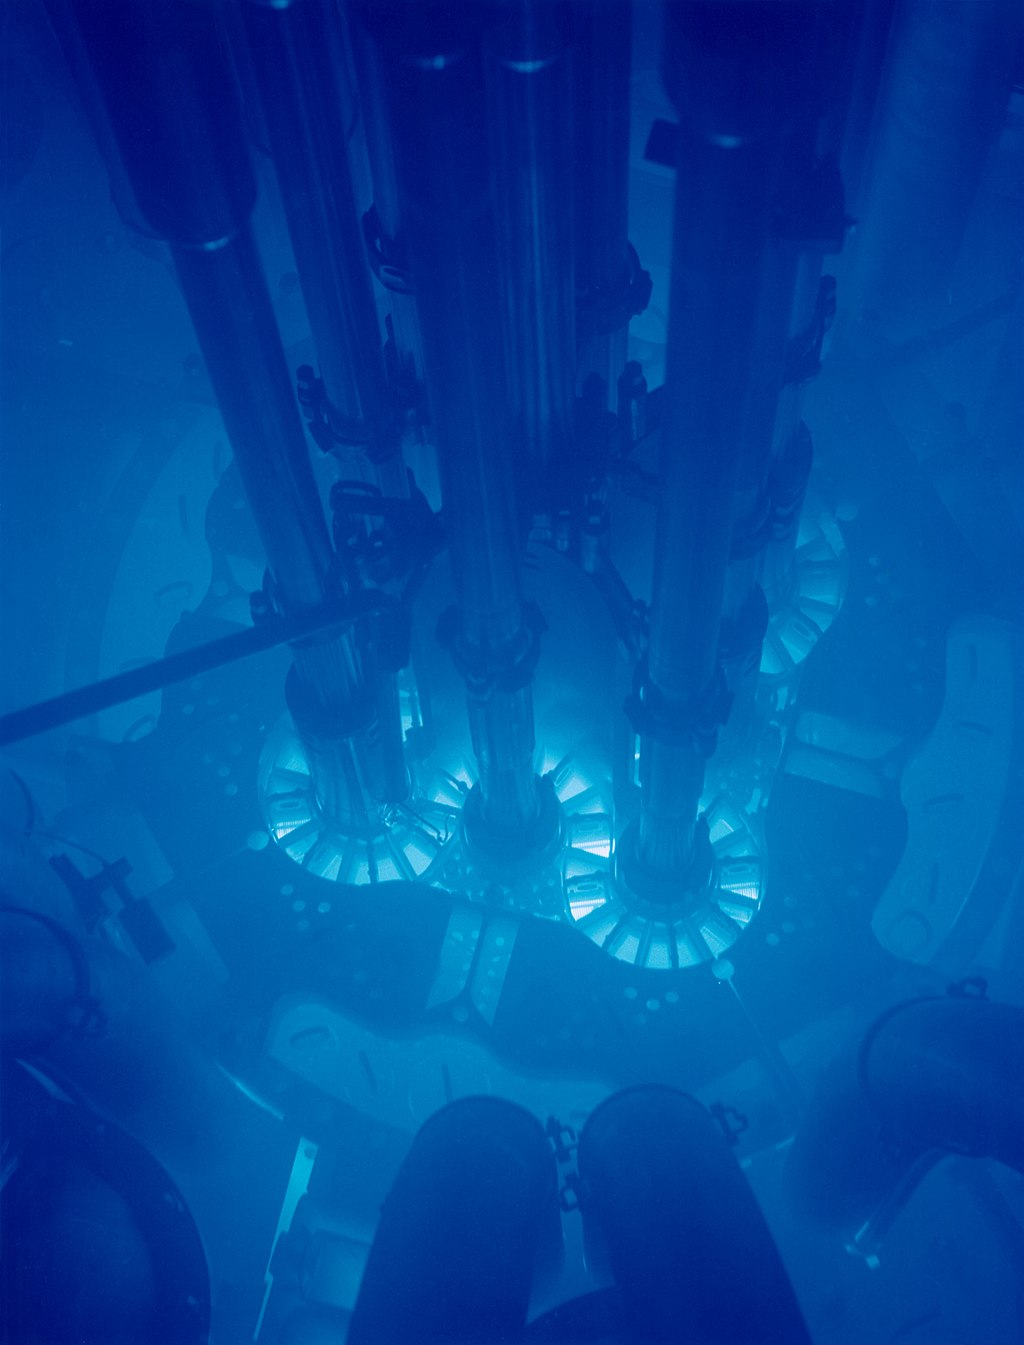
\includegraphics[height = 0.8\textwidth]{Cherenkov-reactor.jpg}}{\textcopyright Argonne National Laboratory\\Advanced Test Reactor core, Idaho National Laboratory}
	\caption{Cherenkov radiation in a nuclear reactor}
	\label{figure: Cherenkov reactor}
\end{minipage}
\hspace{0.05\textwidth}
\begin{minipage}{0.45\textwidth}
	\centering
	\copyrightbox[r]{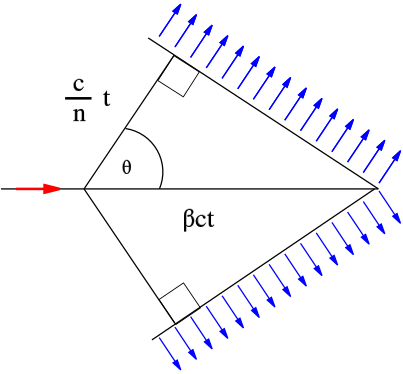
\includegraphics[height = 0.8\textwidth]{Cherenkov.png}}{\textcopyright Arpad Horvath}
	\caption{Diagrammatic representation of Cherenkov radiation}
	\label{figure: Cherenkov illustratie}
\end{minipage}
\end{minipage}
\end{figure}
% =====================================================================
% End matter
% =====================================================================
\newpage
%----------------------------------------------------------------------------------------
%	REFERENCE LIST
%----------------------------------------------------------------------------------------
\bibliography{sources}
\bibliographystyle{plain}

\end{document}
